\begin{center}
    \Large{\textbf{Теоретична частина}}    
\end{center}

\vspace{1mm}

Кільця Ньютона утворюються при інтерференції світлових хвиль, відбитих
від границь тонкого повітряного прошарку, який знаходиться між опуклою
поверхнею лінзи і плоскою скляною пластинкою (рис.1). Спостереження
ведеться у відбитому світлі.


\begin{wrapfigure}{r}{0.4\textwidth}    
    \centering
    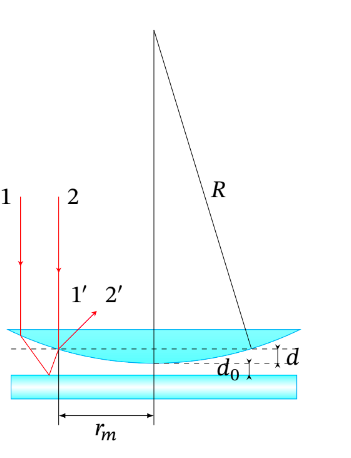
\includegraphics[width=.4\textwidth]{assets/illustation.png}
    \caption{Утворення кілець Ньютона}
    \vspace{0.5cm}
\end{wrapfigure}


Нехай на систему згори падає монохроматичний 
паралельний пучок променів. Частина
променів (промінь 1 на рис. 1 ) відбивається 
від верхнього краю пластини, а інша
частина(промінь 2 на рис. 1) від нижнього краю лінзи.
Промені $1^{'}$ та $2^{'}$ когерентні, але між ними
виникає різниця ходу. Роль тонкої плівки
виконує повітряний проміжок між пластиною
та лінзою.Нехай на систему згори падає 
монохроматичний паралельний пучок променів.

В першому наближені, як що знехтувати невеликим нахилом
променів у повітряному зазорі, геометрична різниця дорівнює

\begin{equation} \label{eq:1}
    \delta^{'} = 2(d_0 + d)
\end{equation}

де $d_0$ - товщина зазору в місці контакту лінзи та пластини, яка може бути як
додатною, наприклад, за наявності часток пилу між лінзою та пластиною, який
викликає деформацію; $d_0 + d$ - товщина повітряного зазору на відстані $r_m$ від
центру лінзи. Для того, щоб визначити повну різницю ходу $d$ треба прийняти до
уваги зміну фаз світлової хвилі під час відбиття від гранці поділу скло-повітря,
коли показник заломлення першого середовища більше за показник заломлення
другого, та під час відбиття від гранці повітря-скло, коли навпаки показник
заломлення першого середовища менше за показник заломлення другого. Відомо,
що для електричного вектора у першому випадку відбиття відбувається без
зміни фаз, а в другому призводить до зміни фаз на $\pi$; фаза магнітного вектора,
навпаки,змінюється на $\pi$ тільки під час першого відбиття. Таким чином, промені
1 і 2 набувають різниці фаз $\pi$, що відповідає додатковій різниці ходу $\frac{\lambda}{2}$,
а повна різниця ходу:

\begin{equation} \label{eq:2}
    \delta = 2(d_0 + d) + \frac{\lambda}{2}
\end{equation}


Якщо форма лінзи близька до сферичної з радіусом кривизни $R \gg r_m$,
то з геометричних міркувань $ r^2_{m} = 2Rd $ і:

\begin{equation} \label{eq:3}
    \delta = \frac{r^2_m}{R} + 2d_0 + \frac{\lambda}{2}
\end{equation}

Якщо повна різниця ходу дорівнює $ \lambda \left( m + \frac{1}{2} \right) $,
то промені 1 і 2 гаситимуть один одного і спостерігатимуться
темні плями(кільця). Радіус цих кілець легко розрахувати за формулою:

\begin{equation} \label{eq:4}
    r^2_{тем} = R(\lambda m - 2d_0)
\end{equation}

Аналогічно, для радіуса світлих кілець маємо:

\begin{equation} \label{eq:5}
    r^2_{світ} = R(\lambda m - 2d_0 - \frac{\lambda}{2})
\end{equation}

Отже, за графіком залежності $r^2(m)$ від номеру кільця можна визначити
радіус кривизни лінзи, а також величину проміжку в місці контакту.
